\chapter{Bilancia di Cavendish}
\section{Introduzione}
\subsection{Oggetto della ricerca}
Misurazione della costante di gravitazione G mediante la bilancia di Cavendish.
\subsection{Proprietà geometriche dei corpi e strumentazione}

\begin{tabular}{ll}
m=38.3$\pm$0.2 g & massa sfere piccole\\
M=1500$\pm$10 g	 & massa sfere grandi\\
r=9.53 mm & raggio sfere piccole\\
R=31.9 mm & raggio sfere grandi\\
L=5.50m & distanza schermo-bilancia \\
$m_c\cong 2m$ & massa manubrio\\
b = 46.5 mm &\\
d = 50 mm &\\
\end{tabular}


\begin{center}
 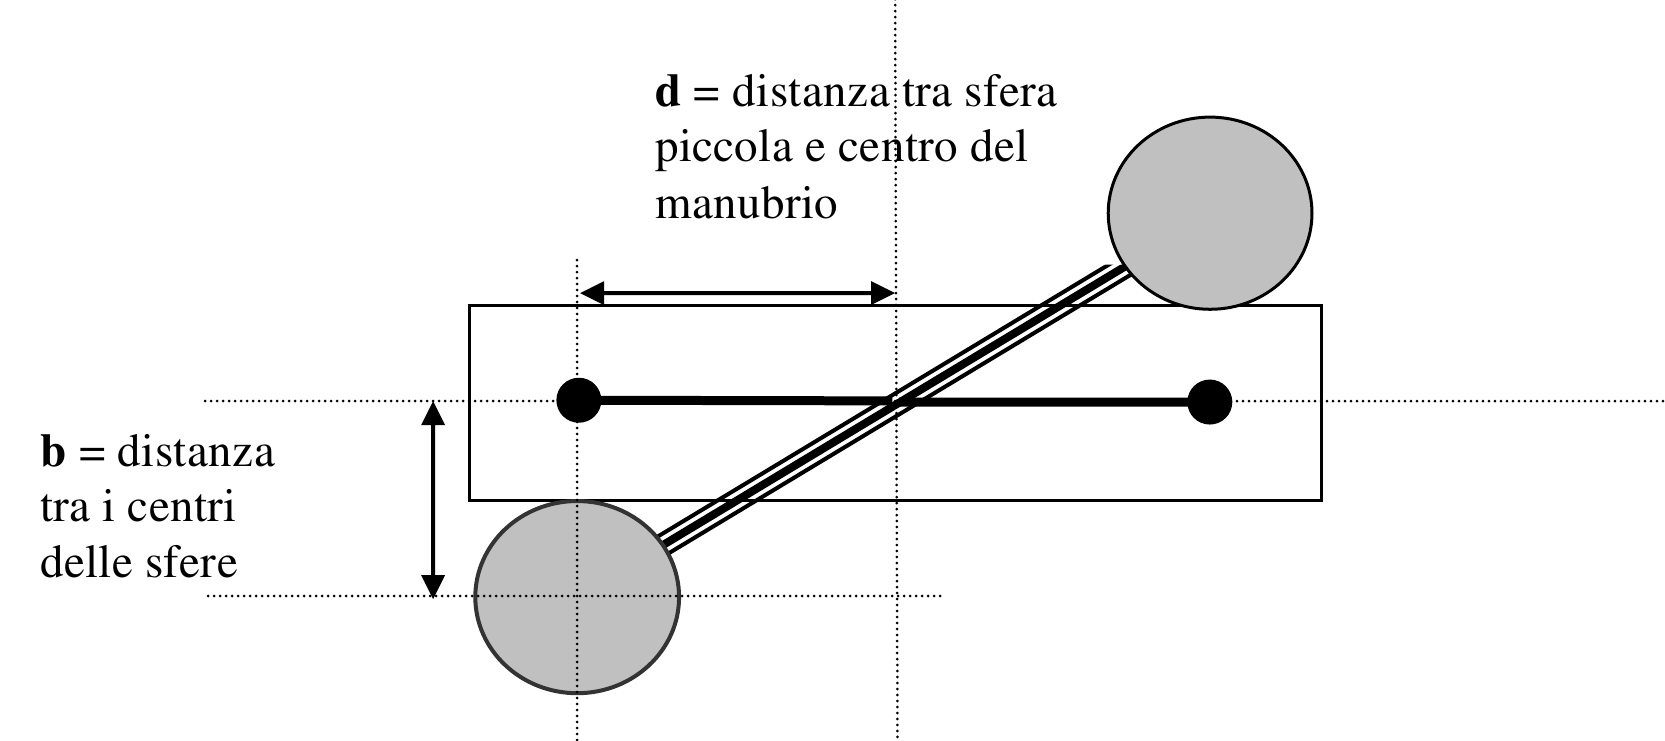
\includegraphics[scale=0.25]{../grafici/cavendish/schema.png}
\end{center}

Il momento d'inerzia $I$ del corpo si calcola:

$$ I=2m(d^2+2/5r^2) = 1.94283 \cdot 10^{-4} kg\cdot m^2$$
L'incertezza sul momento di inerzia è dell'ordine di $10^{-6}$, ed è perciò trascurabile. 
\subsection{Metodo in breve}
La bilancia di Cavendish è uno strumento estemamente sensibile utilizzato per misurare forze di bassissima entità. Il principio su cui si basa è quello dell'equilibrio tra due momenti torcenti: quello della forza di gravità e quello dovuto alla torsione del filo. Questo equilibrio non si raggiunge istantaneamente, ma è necessario attendere un certo tempo, entro il quale il pendolo oscillerà (in modo smorzato).

Per trovare la posizione di equilibrio basterà ricercare una media (mobile) tra i le posizioni di massimo e di minimo.

\begin{center}
 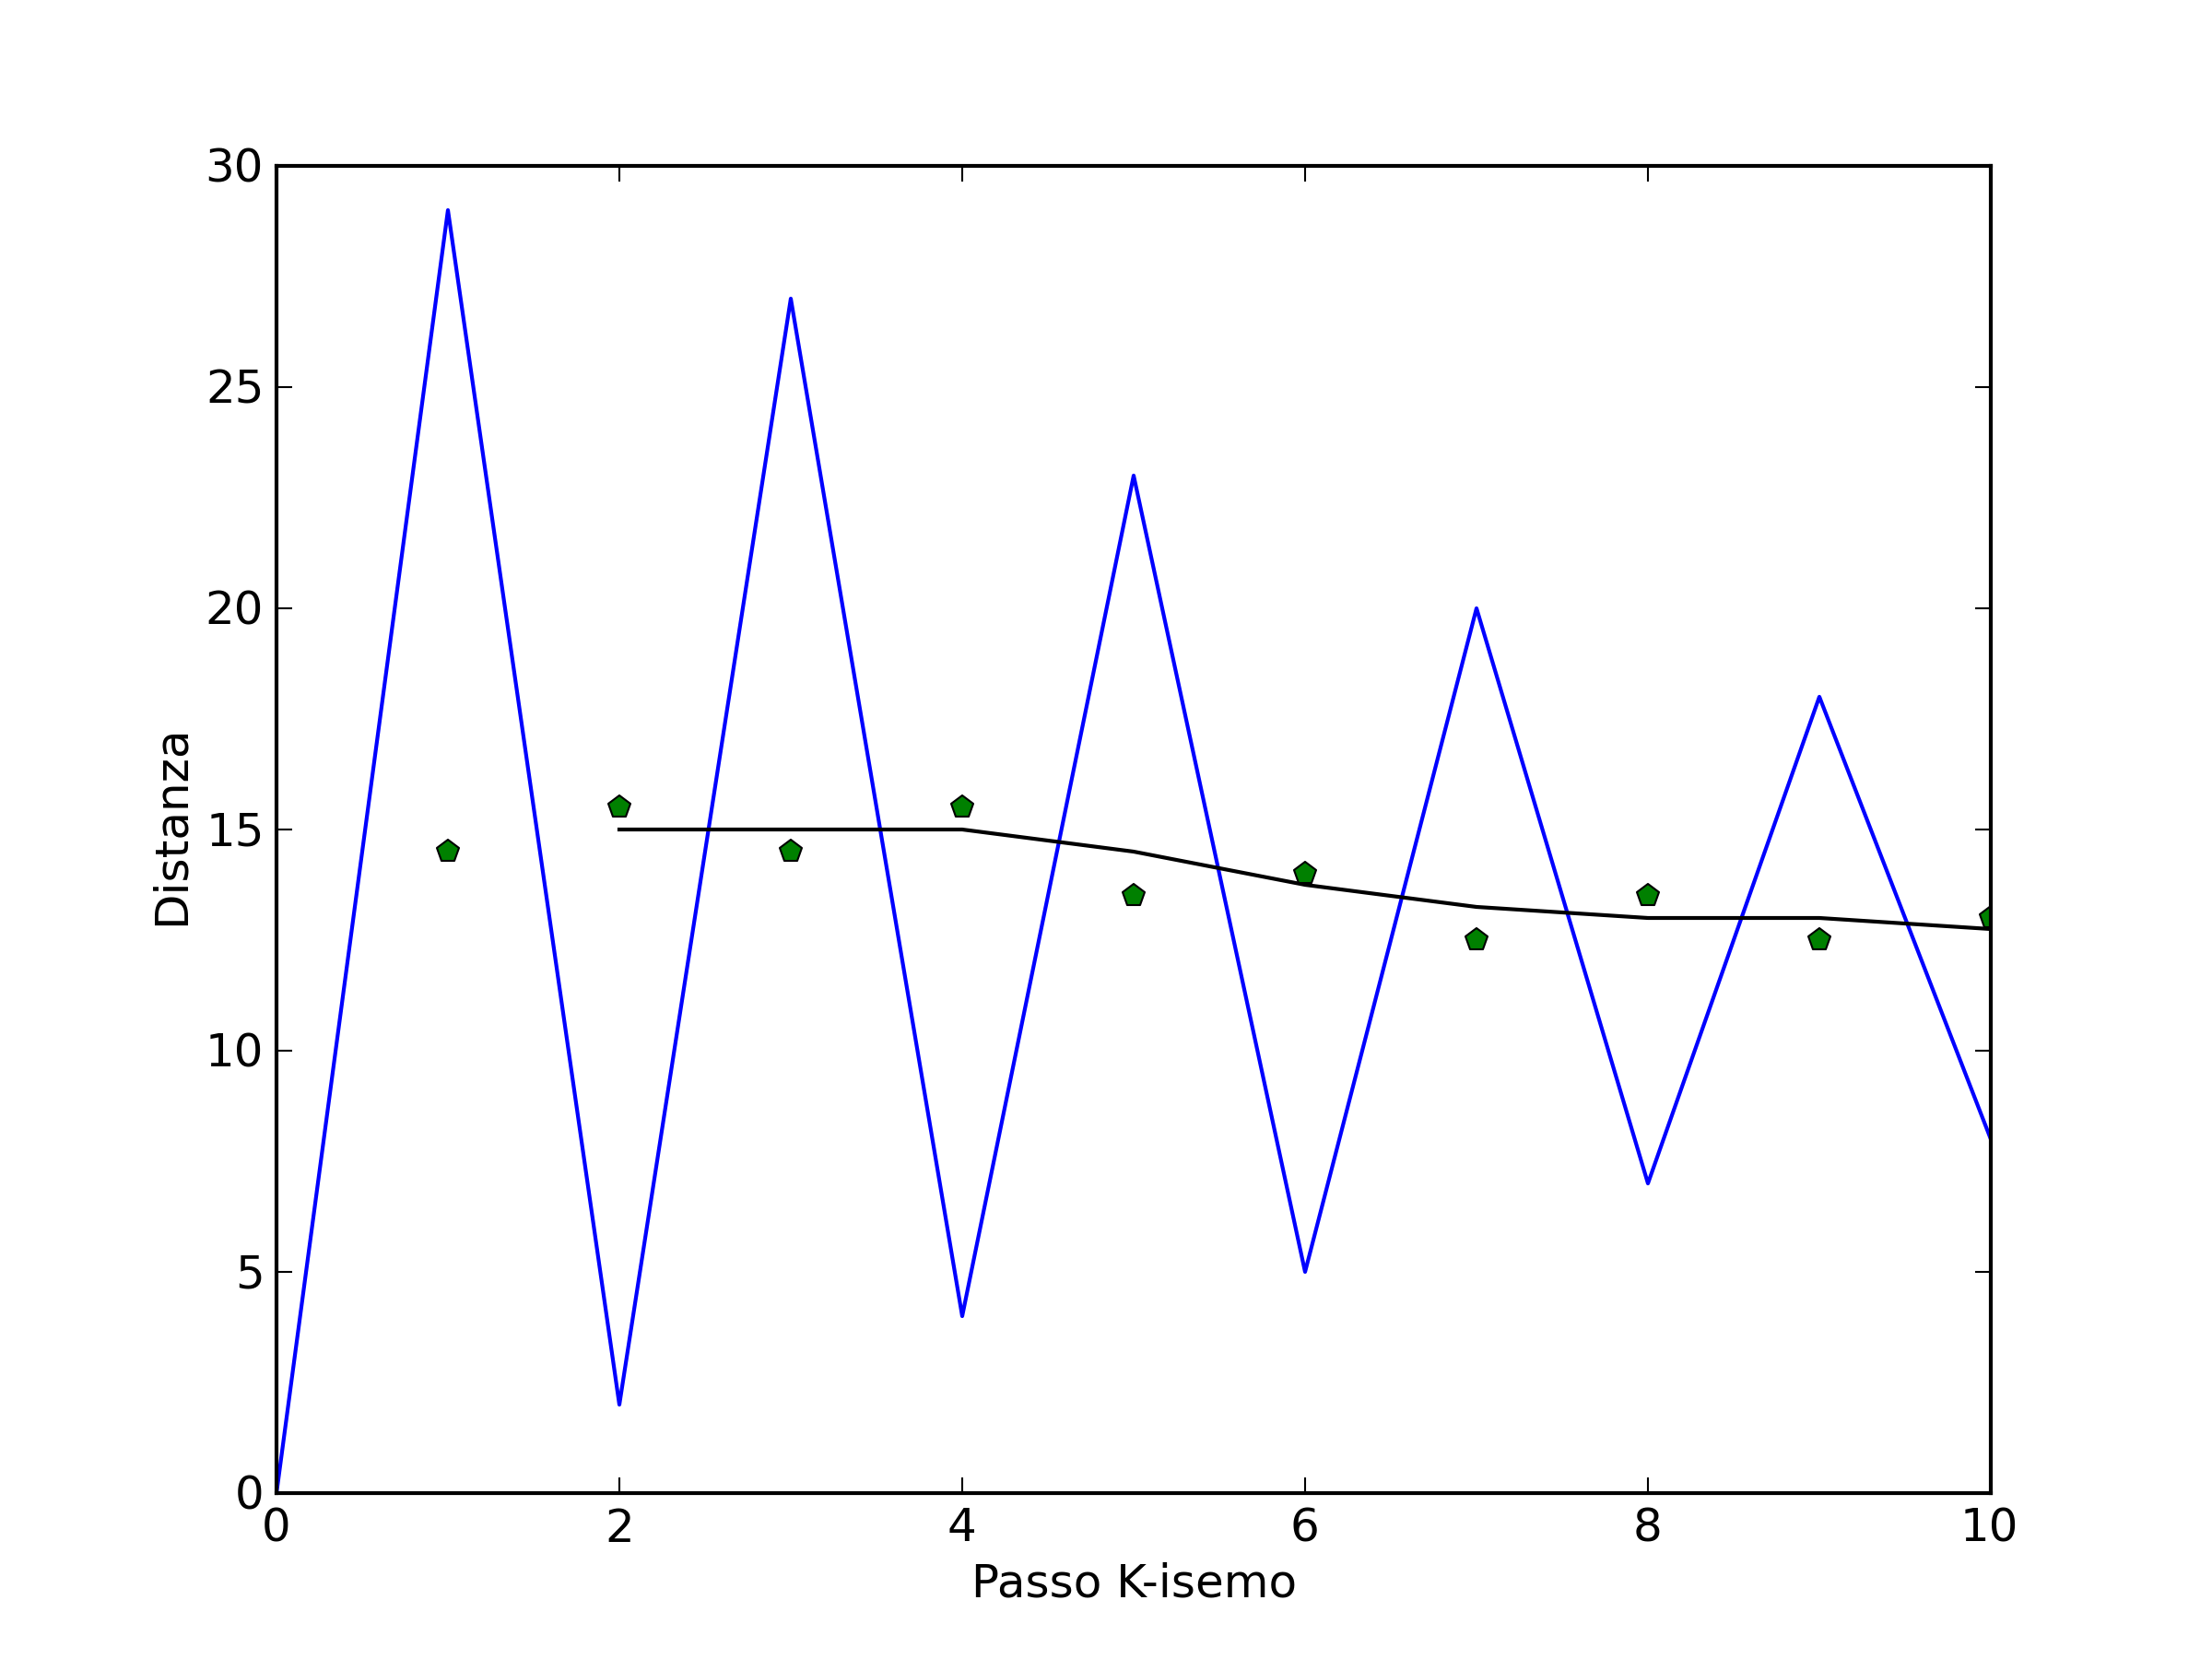
\includegraphics[scale=0.50]{../grafici/cavendish/oscillazioni.png}
\end{center}

Essendo le oscillazioni del pendolo molto piccole, queste vengono amplificate grazie a un laser, che viene fatto incidere sul pendolo, e viene riflesso su di una parete distante circa 5.50 m.

La misurazione sulla posizione di equilibrio e in generale sulla posizione del pendolo vengono effettuate su di un nastro di carta graduata attaccata alla parete.


\section[Misura di k e theta]{Misura $k$ e $\theta$}
L'incertezza relativa allo strumento per la misurazione del periodo è trascurabile rispetto l'entità della misura. Non è così per quella da attribuire allo sperimentatore, che è infatti molto elevata.

Il periodo misurato è dunque ottenuto come media di 5 periodi. L'incertezza è la massima stimata e dipende interamente dallo sperimentatore.

$$T = 513 \pm 20 \ s$$

Per ricavare $k$, ricordiamo che:
$$T^2 = 4 \pi^2 \frac{I}{k}$$
Quindi
$$k = 4 \pi^2 \frac{I}{T^2} = 2.84 \cdot 10^{-8}\ kg\cdot m^2\cdot{s}^{-2}$$
Per quanto riguarda $\theta$, chiamando $s_1$ la prima posizione di equilibrio e $s_2$ la seconda, si ha che:
$$ tan(4\theta) = \frac{s_1-s_2}{L} $$
dove $s_1-s_2$ vale 0.115 m. Si misura $4\theta$ perché la rotazione di $\pi/2$ delle masse più grandi fornisce una rotazione della bilancia pari a $2\theta$ rispetto alla posizione di equilibrio, che va raddoppiata, misurando noi l'angolo riflesso.
$$ \theta = \frac{arctan(\frac{s_1-s_2}{L})}{4} \simeq 5.23 \cdot 10^{-3} rad $$
Inoltre, chiamamdo $F_G$ la forza di attrazione tra una sferetta piccola e quella grande più vicina, si ha che:
$$ \tau_G = 2dF_G = G\frac{mM}{b^2}2d $$
ma per ipotesi
$$ \tau_T = -k\theta = -\tau_G $$
$$ G\cdot\frac{2mMd}{b^2} = k\theta $$
dunque:
$$G = \frac{k \theta b^2}{2mMd} = 5.733 \cdot 10^{-11}\ {m}^3\cdot {kg}^{-1}\cdot{s}^{-2}$$

\section{Analisi dati} 

Correzione:
Bisogna applicare una correzione a $G$, dovuta dall'attrazione che non è stata considerata, tra le sferette piccole e le masse più lontane, che tende a fare ruotare il pendolo in senso opposto. Infatti, questa forza ($F_{G_2}$) fornsce un contributo negativo, e dunque noi con l'esperimento in realtà abbiamo misurato una forza data da:

\begin{equation}\label{eq:fgrav}
 F_{G'} = F_G - F_{G_2}
\end{equation}

(nota: per chiarezza abbiamo preferito $G_t$ come abbreviazione il valore vero (corretto) di $G$, per non confonderla con $G'=G$ che abbiamo misurato prima)
Dunque, non abbiamo misurato il valore vero di $G$, ma un'altro valore, $G'$. Valendo però la relazione \ref{eq:fgrav}, $G_t$ e $G'$ sono legati da una relazione:

\begin{eqnarray*}
G'\cdot\frac{mM}{b^2} & = & G_tmM(\frac{1}{b^2} - \frac{1}{b^2+4d^2}) \\
                      & = & G_t\frac{mM}{b^2}(1 - \frac{b^2}{b^2+4d^2}) \\
\end{eqnarray*}

e quindi:
$$ \frac{G'}{G_t} = 1-\frac{b^2}{b^2+4d^2} = 0.822$$
sicché
$$ G_t = \frac{G'}{0.822}$$
Inoltre:

$$ G_t = 1.216\cdot \frac{\theta k b^2}{2mMd} = 6.9723\cdot 10^{-11}\ {m}^3\cdot {kg}^{-1}\cdot{s}^{-2}$$
